\documentclass{standalone}
\usepackage{tikz}
\usetikzlibrary{calc}
\begin{document}
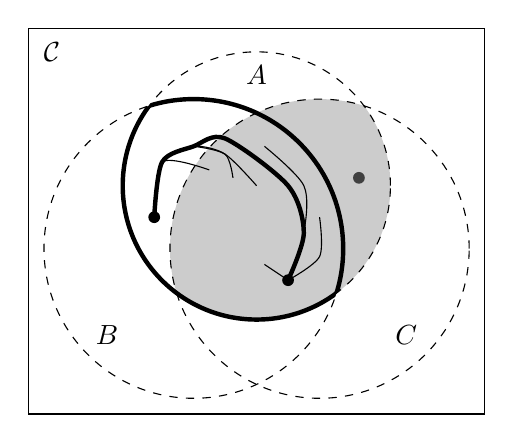
\begin{tikzpicture}

\draw (0,0) rectangle (5.8,4.9);

\coordinate (x) at (2.9,2.9);
\coordinate (y) at (2.1,2.1);
\coordinate (z) at (3.7,2.1);

\def\circlex{(x) circle (1.7)}
\def\circley{(y) circle (1.9)}
\def\circlez{(z) circle (1.9)}

% XnZ
\begin{scope}
   \clip \circlex;
   \fill[color=black!20] \circlez;
\end{scope}

% XnY
\begin{scope}
   \clip \circlex;
   %\fill[pattern=horizontal lines] \circley;
   \draw[ultra thick] \circley;
\end{scope}
\begin{scope}
   \clip \circley;
   \draw[ultra thick] \circlex;
\end{scope}

\draw[dashed] \circlex;
\draw[dashed] \circley;
\draw[dashed] \circlez;

\node (clab) at (0.3,4.6) {$\mathcal{C}$};
\node (xlab) at ($ (x) + (0,1.4) $) {$A$};
\node (ylab) at ($ (y) + (-1.1,-1.1) $) {$B$};
\node (zlab) at ($ (z) + ( 1.1,-1.1) $) {$C$};

\node[circle,fill=black,inner sep=1.5] (p1) at (1.6,2.5) {};
\node[circle,fill=black,inner sep=1.5] (p2) at (3.3,1.7) {};
\node[circle,fill=black!75,inner sep=1.5] (p3) at (4.2,3) {};

\draw plot [smooth] coordinates {
  (p1) (1.7,3.2) (2.3,3.1)};
\draw plot [smooth] coordinates {
  (p1) (1.7,3.2) (2.1,3.4) (2.5,3.3) (2.6,3.0)};
\draw plot [smooth] coordinates {
  (2.1,3.4) (2.5,3.3) (2.9,2.9)};
\draw plot [smooth] coordinates {
  (p2) (3.0,1.9)};
\draw plot [smooth] coordinates {
  (p2) (3.7,2.0) (3.7,2.5)};
\draw plot [smooth] coordinates {
  (p2) (3.5,2.3) (3.5,2.9) (3.0,3.4)};
\draw[ultra thick] plot [smooth] coordinates {
  (p1) (1.7,3.2) (2.1,3.4) (2.5,3.5) (3.3,2.9) (3.5,2.3) (p2)};

\end{tikzpicture}%
\end{document}
